\documentclass[review=false, sigchi]{acmart}

\usepackage{listings}
\usepackage{color}
\usepackage{pgfplots}
\usepackage{subfig}

\raggedbottom
\acmConference[IWOCL'20]{International Workshop on OpenCL}{April 27--29, 2020}{Munich, Germany}
%\editor{John B. Appleseed}
\title[Architecture Independent Memory Access Pattern Analysis]{Characterising Optimisations to Memory Access Patterns using Architecture Independent Program Features}

\author{Aditya Chilukuri}
\email{aditya.chilukuri@anu.edu.au}
\affiliation{%
	\institution{Australian National University}}

\author{Josh Milthorpe}
\email{josh.milthorpe@anu.edu.au}
\affiliation{%
	\institution{Australian National University}}

\author{Beau Johnston}
\email{beau.johnston@anu.edu.au}
\affiliation{%
	\institution{Australian National University}}

%\acmVolume{10} %TODO
%\acmNumber{10} %TODO
%\acmArticle{10} %TODO
\acmYear{2020}
\acmMonth{6}
\acmPrice{15.00}

\keywords{Architecture Independent Analysis, Heterogenous Computing, Workload Characterisation, Memory Access Patterns} %TODO

\definecolor{dkgreen}{rgb}{0,0.6,0}
\definecolor{gray}{rgb}{0.5,0.5,0.5}
\definecolor{mauve}{rgb}{0.58,0,0.82}

\lstset{frame=tb,
	language=C,
	aboveskip=3mm,
	belowskip=3mm,
	showstringspaces=false,
	columns=flexible,
	basicstyle={\small\ttfamily},
	numbers=none,
	numberstyle=\tiny\color{gray},
	keywordstyle=\color{blue},
	commentstyle=\color{dkgreen},
	stringstyle=\color{mauve},
	breaklines=true,
	breakatwhitespace=true,
	tabsize=3,
	numbers=left
}

\begin{document}

	\begin{abstract}
	This paper addresses the challenge of profiling a code base to help programmers effectively optimise their codes for high performance.
	Current methods of analysing program behaviour have largely relied on performance counters on various architectures to provide architecture dependent metrics of code behaviour. 
	However, if workload characteristics are tied to architectural features specific to a particular system, these analysis frameworks may not generalise to alternative or future systems.
	Considering the trend towards heterogeneous computing, we work towards a framework to guide developers in optimising codes for any given hardware target using the architecture independent workload characterisation (AIWC) tool -- specifically in profiling memory access patterns of code. 
	Metrics must be easily interpreted and conceptually linked to patterns in hardware-specific memory access optimisations.
	To this end we propose, implement and analyse the addition of two new metrics to AIWC and present a new approach to profile spatial locality intrinsic to parallel codes.
	The improvements suggested to AIWC will help HPC developers better understand memory access patterns of complex codes, a crucial step in guiding optimisation of codes for arbitrary hardware targets.
	\end{abstract}
	\maketitle	
	
	\section{Introduction}
	
	High-performance computing (HPC) systems are increasingly incorporating a multitude of heterogeneous compute elements. Single nodes on supercomputers now comprise of traditional CPUs and multiple accelerators such as GPUs, Field Programmable Gate Arrays (FPGAs), and many-integrated-core devices (MICs). The development of high bandwidth interconnects between compute devices supports tight integration between multiple devices of different types on the same compute node.
	
	The OpenCL programming language is designed to support modern HPC software engineers in writing code that executes on multiple hardware targets. 
	%It is possible for an engineer to write highly thread-divergent logical analysis code aimed at traditional CPUs; parallelisable data crunching kernels aimed at GPUs; and code to satisfy specialised computational requirements aimed at FPGAs -- all in a single code base using OpenCL. 
	The language provides support for individual \emph{kernels}, portions of parallelisable codes that make up a HPC code base, to be executed independently on diverse hardware targets such as traditional CPUs, GPUs and FPGAs \cite{khronosopenclworkinggroup2011opencl}. This gives HPC software developers greater flexibility by allowing codes aimed at a range of hardware targets to be written in a single programming language environment.
	
	Application codes differ in resource requirements, control structure and available parallelism. Similarly, compute devices differ in number and capabilities of execution units, processing model, and available resources. These heterogeneous computing environments present opportunities for software engineers and HPC integrators to design highly optimised systems with multiple kernels executing on hardware targets best suited for the diverse computational tasks performed by these kernels \cite{spafford2010maestro}.	However this opportunity raises the twin challenges of deciding on the right hardware target for complex kernels; and optimising codes to run on these diverse architectures. Our work is directed at helping developers tackle the latter of these two problems.
	
	Modern computer architectures have suffered from the exponential growth in computational speeds being unmet by proportional increases in memory speeds\cite{hennessycomparch}. Memory accesses pose larger bottlenecks to performance as applications' demand for main memory scales with the arithmetic capability of computer systems. To mitigate this latency, modern CPU designs have employed a wide range of cache technologies to reduce main memory accesses using the principle of \emph{spatial locality}: the idea that programs repeatedly access memory addresses in close locality. On the other hand, GPUs rely on hardware multithreading to hide memory latency, and their architectures favour ALU capability over sophisticated logic to manage a cache hierarchy and out-of-order execution. As a result, the performance of kernels on CPUs and GPUs alike is strongly dependent on memory access patterns intrinsic to the code. % We discuss the memory model design and the manufacturer recommended optimisations for NVIDIA GPUs in later sections..
	
	%We demonstrate the effectiveness of an architecture-independent analysis of codes in determining ... Our work guides optimisation efforts for OpenCL codes running on increasingly diverse hardware by examining the current state of the art in architecture-independent metrics for memory access patterns. 
	
	
	%What we did briefly
	Our aim in this paper is to develop a framework to guide HPC software engineers in hardware dependent code optimisation -- specifically by guiding the improvement of codes' memory access patterns. We provide examples of manufacturer recommended code optimisations to improve memory access patterns on the target architecture, and examine these using AIWC \cite{beauaiwc}, a state of the art architecture-independent code analysis tool for parallel workloads. Our work highlights the benefits and challenges arising from an architecture independent analysis of memory based program characteristics. We suggest the addition of two new metrics to AIWC to better characterise these memory-based optimisations. We measure the presented codes using the new metrics and discuss the metrics' effectiveness in capturing the essence of the optimisations performed. With these improvements, we show that AIWC is better suited to be used by HPC software engineers in guiding optimisation of their codes. 
	
	The structure of this paper is as follows. In section \ref{motivating example}, we use the example of GPU matrix multiplication code to showcase the specific vendor recommended optimisations our work aims to measure. In section \ref{related work} we discuss how AIWC and its precursors profiled memory access patterns in an architecture independent fashion, and relevant architecture dependent approaches to memory access profiling. Then in section \ref{method} we provide a methodology to critically examine AIWC, the current state of the art architecture independent workload characterisation tool. In section \ref{results} we measure the accuracy of AIWC in profiling the impact of performance optimisations to various OpenCL codes. In section \ref{discussion} we suggest new methods to accurately capture code patterns correlating to hardware specific memory optimisations. Finally, in section \ref{future work} we discuss further avenues to extend our work and conclude.
	
	\section{Motivating Example} \label{motivating example}
	
	We aim to capture the essence of vendor recommended optimisations for target architectures in our metrics. We demonstrate the optimisation strategies being analysed by presenting a simple unoptimised matrix multiplication kernel for input square matrices of order $N$, and then improve the memory access patterns of this kernel by incrementally performing optimisations recommended in the CUDA Optimisation Handbook \cite{cudaoptimisation} for NVIDIA GPUs. These incrementally optimised OpenCL codes are then analysed using AIWC to determine the accuracy in profiling favourable memory access patterns of the current framework and the proposed extensions to AIWC.
	
	\subsection{Simple unoptimised matrix multiplication}
	
	The unoptimised matrix multiplication kernel presented in Appendix \ref{simpleMultiply} is used as a baseline to validate the performance improvements measured from each following optimisation. Each thread of the kernel computes the $(globalRow, globalCol)$ element of matrix $C$ by reading the appropriate row and column from matrices $A$ and $B$ respectively.
	
	\subsection{Using Shared Memory to Coalesce Global Memory Access to Matrix A} 
	
	We first notice that the number of global memory accesses to matrices A and B increases at an order $O(N^3)$ with respect to matrix size $N$. Global memory is typically located off-chip and accesses induce large delays. NVIDIA GPUs coalesce global memory loads and stores issued within thread-groups into as few DRAM transactions as possible. Multiple global memory loads and stores are coalesced into a single transaction when certain device specific conditions are met. On most NVIDIA GPUs, data accesses are coalesced when multiple requests are made for memory locations from the same cache-line in global memory \cite{cudamanual}. Appendix \ref{coalescedAMultiply} contains the \texttt{coalescedAMultiply} kernel, which coalesces accesses to matrix $A$ by storing \emph{tiles}, or square blocks, of $A$'s values into shared memory. 
	
	% 9.2.1.2: Misaligned access pattern
	
	\subsection{Using Shared Memory to store Tiles of Matrix B} 
	
	The code is further optimised by improving how the previous \texttt{coalescedAMultiply} kernel handles accesses to Matrix $B$. While each thread in coalescedAMultiply accesses only a single element of matrix $A$ from global memory, each thread accesses a full column of matrix $B$. The repeated reads to elements of matrix $B$ across multiple threads can be alleviated by reading tiles from matrix $B$ into shared memory. Appendix \ref{coalescedABMultiply} contains the \texttt{coalescedAB} kernel which performs this optimisation.
	
	\subsection{Optimising handling of shared memory} 
	
	NVIDIA shared memory is divided into multiple banks -- stored in independent memory modules -- to allow parallel accesses to shared memory. Bank conflicts occur when shared memory in the same bank is accessed concurrently. The code in \texttt{coalescedAB} kernel is further optimised by implicitly transposing tiles of Matrix $A$ while loading from global memory. This improves memory bank utilisation during reads to shared memory tiles are performed during the necessary computation. The \texttt{coalescedABT} kernel demonstrates this optimisation by modifying lines 20,21 of \texttt{coalescedAB} to:
	
	\begin{lstlisting}[firstnumber=20]
		ASub[localCol][localRow] = A[tiledRow];
		BSub[localRow][localCol] = B[tiledCol];
	\end{lstlisting}
	
	
	\subsection{Alignment of Memory Allocation}
	
	Memory access alignment is important to best utilise all parts of GPU memory architecture. Global memory buffer alignment can allow threads to access blocks of global memory aligned to the nearest cache line. This enables coalescing of memory accesses. If buffers are misaligned, parallel memory requests may cross over cache lines, and may double the number of slow global memory accesses needed as demonstrated in figures \ref{fig: Simple memory alignment} and \ref{fig: Simple memory misalignment}.
	
	\begin{figure}[h]
		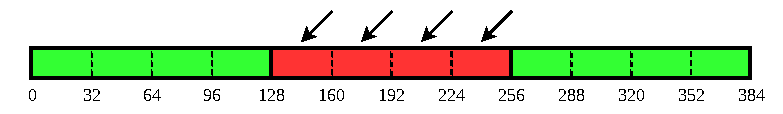
\includegraphics[width=\linewidth]{aligned_access_coalescing.pdf}
		\caption{All threads access memory aligned to nearest cache line in parallel \cite{cudaoptimisation}}
		\label{fig: Simple memory alignment}
	\end{figure}
	
	\begin{figure}[h]
		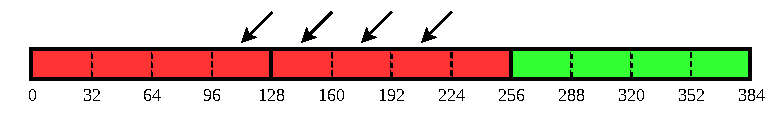
\includegraphics[width=\linewidth]{misaligned_access_coalescing.pdf}
		\caption{Unaligned sequential memory addresses fit in two cache lines \cite{cudaoptimisation}}
		\label{fig: Simple memory misalignment}
	\end{figure}
	
	A similar principle applies when using shared memory. Bank conflicts may be reduced by aligning allocations of shared memory buffers. The \texttt{alignedABT} kernel improves the alignment of shared memory tiles in \texttt{coalescedABT}. An arbitrary large alignment value of 4096 is chosen as it is larger than the size of modern hardwares' cache lines and attributed to the local array declarations in the existing code as shown below.
	
	\begin{lstlisting}
		__local float aTile[TILE_DIM][TILE_DIM] __attribute__ ((aligned(4096)));
		__local float bTile[TILE_DIM][TILE_DIM] __attribute__ ((aligned(4096)));
	\end{lstlisting}
	
	All the examples above are an incomplete listing of optimisation strategies developers can perform to code targeted at NVIDIA GPUs. We analyse the correlations between the collected AIWC metrics for each of these kernels and our conceptual understanding of GPU memory optimisations. This allows us to examine how effectively our methodology uncovers underlying bottlenecks and guides optimisation efforts.
	
	\flushbottom
	\section{Related Work} \label{related work}
	
	Hoste and Eeckout \cite{hoste2007microarchitecture} show that while conventional architecture dependent characteristics are useful in locating performance bottlenecks, they can hide the underlying, inherent program behaviour causing performance bottlenecks. A conceptual understanding of the performance characteristics of complex codes is necessary for the programmer to effectively optimise these codes. Architecture dependent characteristics typically include instructions per cycle (IPC), cache and branch prediction miss rates, page faults and DRAM bus data transfer rates. These are typically collected using hardware performance counters available on most target architectures. These performance counters do not serve to guide optimisation beyond highlighting potential bottlenecks \cite{hoste2007microarchitecture, ganesan2008performance}. Further, in many cases, architecture dependent characteristics usually cannot be directly correlated to specific code patterns. For example, the causes of high cache miss rates in the execution of a program are too complex and widely variant on microarchitecture specific features such as cache size, prefetch behaviour and cache placement policies. In summary, we argue that a HPC developer tasked with optimising code for a given hardware target would benefit from architecture-independent metrics of the code that can be conceptually correlated to hardware specific optimisation patterns. Such architecture-independent metrics will effectively guide the HPC developer's workflow in both finding and fixing bottlenecks in code performance.
	
	The Architecture Independent Workload Characterisation (AIWC) tool \cite{beauaiwc} relies on a set of instruction set architecture (ISA)-independent features determined by Shao and Brooks \cite{shao2013isa}. AIWC measures memory based metrics to characterise the target code's memory behaviours. AIWC firstly collects aggregate simple counts such as the (i) total memory footprint, the total number of unique addresses accessed; and (ii) 90\% memory footprint, the number of unique addresses covering 90\% of memory accesses. A small ratio of 90\% memory footprint to total memory footprint correlates to programs accessing the same small subset of memory addresses repeatedly -- which can be linked to increased performance in a cached memory hierarchy.
	
	AIWC also records the global memory address entropy (GMAE), a positive real number corresponding to the randomness of the memory access distribution of a program. To measure locality of memory accesses, AIWC collects the local memory address entropy (LMAE) of memory addresses accessed after dropping $n$ least significant bits of all memory addresses accessed by the program. To calculate this, AIWC collects a frequency distribution of all non-register memory accesses by all threads in the target kernel. Using the collected frequency distribution, AIWC calculates 10 separate local memory address entropy (LMAE) values according to increasing number of least significant bits (LSB) skipped using
	%in the following fashion. The information entropy of the collection of memory addresses accessed, after dropping $n$ LSBs and accounting for the number of memory accesses performed to each address is counted as the $n$-bits skipped LMAE. Given the frequency distribution of memory addresses accessed by the program, 
	the explicit formula for the $n$-bits skipped LMAE:
	
	\begin{equation}
	LMAE_{n-bits} = \sum_{a \in A_n}p_a \log_2(p_a^{-1})
	\end{equation}
	
	\begin{itemize}
		\item $A_n$ is the set of all addresses accessed after skipping $n$ LSBs of each address.
		\item $p_a := \frac{\#access_a}{\#access_{total}}$ is the probability (calculated as relative frequency) at which each memory address is accessed.
	\end{itemize}
	
	LMAE measures the locality of memory accesses performed over the full execution of a program. A steeper drop in entropy with increasing number of bits may correlate to more localised memory accesses over the program's execution.
	
	Limitations of the memory footprint and local memory address entropy values as memory access pattern metrics are further discussed by this work. %TODO: REMOVE?
	
	\subsection{Advancements in Memory Access Pattern Characterisation}
	
	We provide a brief summary of past work in architecture independent program characterisation and Memory Access Pattern analysis:
	
	\begin{itemize}
		\item The Microarchitecture Independent Workload Characterisation Tool (MICA) \cite{hoste2007microarchitecture} was the first microarchitecture independent workload characterisation tool for single threaded programs. 
		\item The Workload ISA-Independent Characterization for Applications (WIICA) \cite{shao2013isa} extends MICA to present a framework to analyse single threaded programs independent of the ISA.
		\item CuMAPz: CuMAPz \cite{kim2011cumapz} is a CUDA memory access profiling tool and the first to present metrics for CUDA codes which can be generalised to any given NVIDIA GPU.
	\end{itemize}
	
	\subsection{MICA}
	
	The MICA framework was developed by Hoste and Eeckout \cite{hoste2007microarchitecture} in response to their findings on the limitations of conventional microarchitecture dependent characteristics. Hoste and Eeckout discovered that performance counter based approaches to profiling codes often struggled in finding underlying program features that map to improved or worsened usage of performance critical hardware features of the target architecture. The MICA framework is a holistic characterisation tool, and thus collects features including instruction mix, instruction-level parallelism, register traffic, data stream strides and branch predictability.
	
	Of these metrics, data stream strides are of particular interest in memory access pattern profiling. MICA's stride length metric measures the distance between consecutive memory accesses in a single threaded application. For CPU architectures running single threaded applications, this metric correlates to the spatial locality of memory accesses -- a measure of how closely bunched are memory access in nearby times. This is directly correlated to cache reuse rates, critical to code performance on CPUs \cite{inteloptimisation}. %Intel optimisation manual.
	
	The MICA approach was tailored for single-threaded applications as the metrics collected rely heavily on Pin instrumentation \cite{luk2005pin}. As such, MICA is unsuited to analysing conventional supercomputing workloads with heavy use of parallelism.

	\subsection{CuMAPz}
	
	Kim and Shrivastava \cite{kim2011cumapz} present CuMAPz, a CUDA memory access pattern analysis tool to guide NVIDIA GPU optimisations. CuMAPz focuses on the problem of improving CUDA application performance using NVIDIA memory-based optimisations. CuMAPz analyses CUDA codes structurally and simulates code execution on the memory hierarchy of specific NVIDIA GPU models.
	
	During the simulated run of the target code, CuMAPz records all memory accesses in various buffers to simulate the global and shared memories on NVIDIA GPUs. Using this detailed simulation data, CuMAPz can estimate the performance critical (i) shared memory data reuse profit, (ii) profit from coalesced access (iii) memory channel skew cost and (iv) bank conflict cost characteristics of the target code.
	
	The simulation environment described in CuMAPz and the attached analysis framework is highly specific to CUDA enabled GPUs. Replicating the CuMAPz framework for all target architectures is challenging. However, CuMAPz is an interesting simulator from the standpoint of this paper's work since it adheres to the core parts of NVIDIA GPUs' memory models in its analysis, while allowing the user to specify their GPU model specific hardware information.
	
	Our approach is an architecture independent analysis of memory access patterns that provides metrics correlating to similar performance critical memory access optimisations as CuMAPz. We aim to further the state of the art by providing a framework to guide developers in optimising OpenCL codes for any given target architecture. To the best our knowledge, none of the previous works present a set of performance metrics that accurately characterise memory access patterns of parallel applications independent of the target architecture.
	
	\section{Methodology} \label{method}
	
	To provide memory access pattern metrics that represent vendor recommended optimisations on GPUs, we improved AIWC by adding a new metric: relative local memory usage. This measures the proportion of all memory accesses from the symbolic execution of the kernel that occurred to memory allocated as \texttt{\_\_local}. On GPUs, this memory address space is mapped to fast on-chip shared memory.
	
	Relative local memory usage is an example of a metric that is useful to measure performance critical access patterns on some architectures such as GPUs, and not others, such as CPUs. CPUs do not typically have a notion of user controlled on-chip memory shared between hardware threads such as NVIDIA GPUs' shared memory. This is a natural consequence of programming for a heterogeneous system. Specific code patterns may translate to performance improvements only on certain hardware.
	
	In the original AIWC tool \cite{beau_johnston_2017_1134175}, global and local memory address entropy (MAE) were calculated using physical addresses of memory used by the Oclgrind simulator back-end of AIWC. This caused irregularities in entropy calculations across multiple runs of the same simulation. We improved the calculation of memory address entropy by using \textit{virtual addresses} to calculate MAE values using an abstract ideal address space on which all memory accesses by the kernel occur. This allows AIWC to accurately abstract over the hardware and ISA-specific differences in memory layouts across the diverse hardware targets.
		
	\section{Results} \label{results}
	
	\begin{figure*}[h!]
		\centering
		\subfloat{
			\centering
			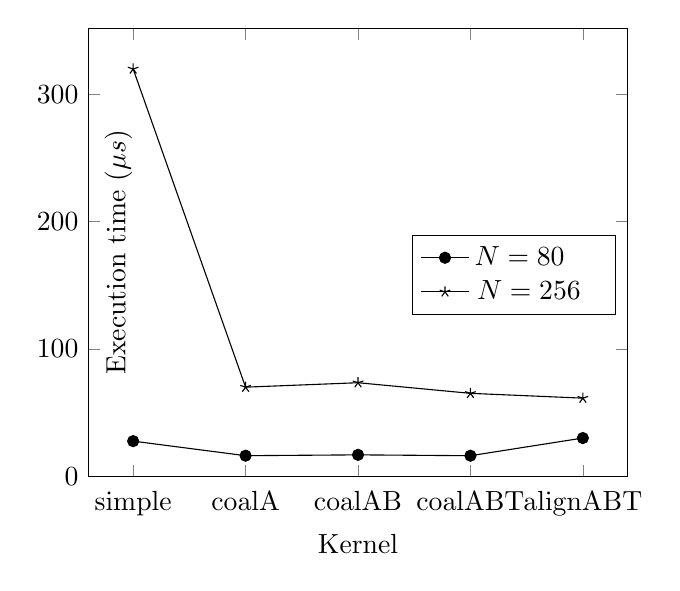
\begin{tikzpicture}
			\begin{axis}[symbolic x coords={simple,coalA,coalAB,coalABT,alignABT},
			xtick={simple,coalA,coalAB,coalABT,alignABT},
			xticklabel style={text height=2ex},
			ymin=0,
			ylabel={Execution time ($\mu s$)}, xlabel={Kernel},
			ylabel style={at={(axis description cs:0.1,.5)},anchor=south},
			legend entries={$N=80\ \ \ \ $,$N=256\ \ $},
			legend style={at={(0.6,0.45)},anchor=west}
			]
			
			\addplot[mark=*] coordinates {
				(simple,27.79)
				(coalA,16.36)
				(coalAB,17.02)
				(coalABT,16.34)
				(alignABT,30.21)
			};
			\addplot[mark=star] coordinates {
				(simple,319.71)
				(coalA,70.12)
				(coalAB,73.60)
				(coalABT,65.27)
				(alignABT,61.50)
			};	
			\end{axis}
			\end{tikzpicture} 
		}
		\subfloat{
			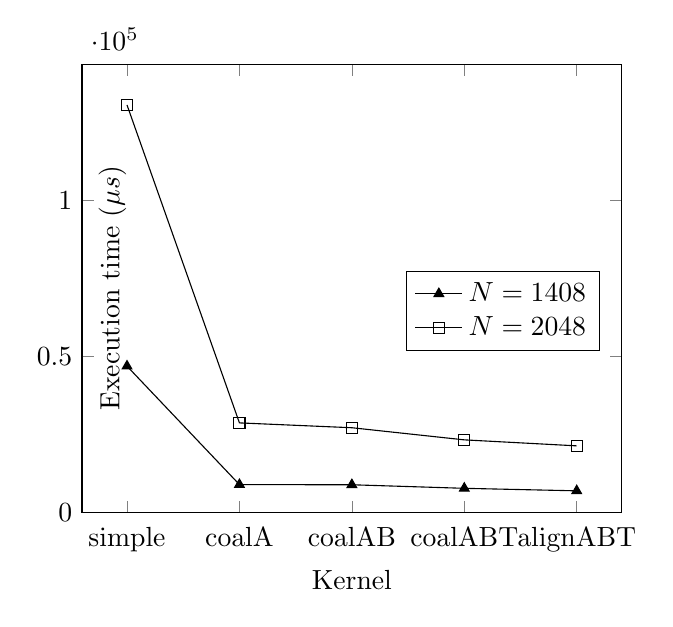
\begin{tikzpicture}
			\begin{axis}[symbolic x coords={simple,coalA,coalAB,coalABT,alignABT},
			xtick={simple,coalA,coalAB,coalABT,alignABT},
			xticklabel style={text height=2ex},
			ymin=0,
			ylabel={Execution time ($\mu s$)}, xlabel={Kernel},
			ylabel style={at={(axis description cs:0.1,.5)},anchor=south},
			legend entries={$N=1408$,$N=2048$},
			legend style={at={(0.6,0.45)},anchor=west}
			]
			
			\addplot[mark=triangle*] coordinates {
				(simple,46901.35)
				(coalA,8948.96)
				(coalAB,8894.74)
				(coalABT,7756.75)
				(alignABT,6951.7773435)
			};
			\addplot[mark=square] coordinates {
				(simple,130601.41)
				(coalA,28722.51)
				(coalAB,27169.72)
				(coalABT,23284.03)
				(alignABT,21363.90)
			};	
			\end{axis}
			\end{tikzpicture} 
		}
		\caption{NVIDIA Tesla P100 Runtime performance of section \ref{motivating example} codes averaged over 100 runs}
		\label{fig: matmul runtime}
	\end{figure*}

	Figure \ref{fig: matmul runtime} shows that across varying problem sizes, the vendor recommended optimisations to the matrix multiplication code lead to increased performance. Note that a matrix size of 80 is small -- overheads attached to optimisation techniques may be causing the observed decrease in performance as some optimisations are performed.

	\begin{table*}[h!]
	\centering
	\begin{tabular}[t]{lrrrrr}
		\toprule
		& simple & coalescedA & coalescedAB & coalescedABT & alignedABT \\ \midrule 
		Total memory footprint        & 196608 & 196608     & 196608      & 196608       & 196608     \\ %\hline
		90\% Memory Footprint         & 118196 & 56176      & 489         & 489          & 489        \\ %\hline
		Global MAE                    & 17.02  & 13.18      & 9.78        & 9.78         & 9.78       \\ %\hline
		LMAE \#bits=3                 & 16.02  & 12.18      & 8.78        & 8.78         & 8.78       \\ %\hline
		LMAE \#bits=10                & 9.02   & 5.18       & 1.78        & 1.78         & 1.78       \\ %\hline
		Relative Local Memory Usage   & 0      & 49.9083    & 94.28       & 94.28        & 94.28      \\ \bottomrule
	\end{tabular}
	\caption{Selection of AIWC\cite{beauaiwc} metrics for 256 $\times$ 256 matrix multiplication}
	\label{matmul aiwc table}
	\end{table*}

	Table \ref{matmul aiwc table} summarises AIWC memory metrics collected for each of the matrix multiply kernels in section \ref{motivating example}. Note that only two LMAE values are shown for brevity. We now analyse the effectiveness of AIWC metrics in profiling the NVIDIA recommended memory optimisations applied to the matrix multiplication kernel.
	
	\textit{Relative local memory usage}: As reliance on NVIDIA GPUs' shared memory increases in each kernel from \texttt{simpleMultiply} to \texttt{coalescedAB}, we find that the ratio of OpenCL local memory usage increases as expected.
	
	\textit{Global and local MAE}: Entropy measurements decrease from \texttt{simpleMultiply} to \texttt{coalescedAB}. This is explained by the optimisations performed incrementally reducing accesses to matrix $A$ and $B$, and instead performing the bulk of computations on smaller tiles in on-chip shared memory. We observe an almost completely uniform distribution of memory accesses in \texttt{simpleMultiply}, where the program makes $N$ loads to each element of $A$ and $B$ with $N$ the dimension of the matrices. The frequency distribution of memory addresses accessed become increasingly non-uniform as we perform less accesses to matrices $A$ and $B$ and offset this by increasing the frequency of accesses to smaller, more localised shared memory buffers. The non-uniformity of relative frequency with which each memory cell is accessed by the program translates directly to decreases in local and global memory entropy values as reliance on small shared memory buffers increases from \texttt{simpleMultiply} to \texttt{coalescedAB}.
	
	\textit{Memory Footprint}: Similar to trends in global and local MAE, we find that the ratio of 90\% memory footprint to total memory footprint decreases from $60.12\%$ for \texttt{simpleMultiply} to $0.25\%$ (\texttt{coalescedAB}). Increased utilisation of shared memory in the optimised kernels means that the shared memory buffers make up a greater proportion of total memory accesses in the program. As the shared memory buffers are small and reused within a workgroup, the memory footprint of the shared memory buffers is also smaller. 
	
	AIWC's metrics strongly reward optimisations that tend to localise memory accesses. Shared memory buffers are typically smaller than global memory arrays when programming for GPUs due to hardware limitations on sizes of shared memory buffers \cite{cudamanual}. However, the metrics currently measured by AIWC do not have a direct causal relation to code patterns that optimise memory accesses on GPUs. The proposed relative local memory usage metric is the first to correspond to a recommended optimisation strategy of using fast on-chip shared memory. Further, we find that all current AIWC metrics do not measure any sizeable difference between \texttt{coalescedAB}, \texttt{coalescedABT} and \texttt{alignedABT} codes. We address the root cause of this -- a lack of temporal information about memory accesses, in the next section.%TODO READ THIS SECTION
	
	\section{Discussion} \label{discussion}
	
	AIWC metrics are inherently lossy. Given the set of metrics calculated for an unknown kernel, we can not reconstruct the kernel based on these metrics. Specifically to memory access pattern analysis, the calculation of memory address entropy of a kernel relies only on the frequency distribution of memory accesses to all addresses accessed by the kernel. We observe that calculation of memory address entropy does not make use of temporal information. The order of sequential memory accesses performed by each thread, as well as addresses requested in parallel by multiple threads in an OpenCL thread group, are both vital in accurately characterising parallel codes.
	
	We propose a new architecture independent metric to measure memory access patterns of parallel programs. The proposed metric is inspired by CuMAPz' direct approaches to measuring optimisation specific characteristics of CUDA codes.
	
	AIWC currently collects a list of all memory accessed by each thread of execution. In the OpenCL programming model, threads within thread groups execute the same code and are allowed to cooperate on \textit{local memory} addresses. We can group together threads by their work groups to align histories of memory accesses of threads in a group to analyse memory accesses performed by thread groups at each logical time step in the symbolic execution of the code. We argue that analysing the accesses occuring at the same logical time step is an accurate, conceptually sound method of predicting the extent of memory access coalescing and bank conflicts we are likely to find upon executing the code on a GPU.
	
	The precise definition of the proposed metric is provided in the following section.
	
	\subsection{A Parallel Spatial Locality Metric}
	
		\begin{figure*}[h!]
		\centering
		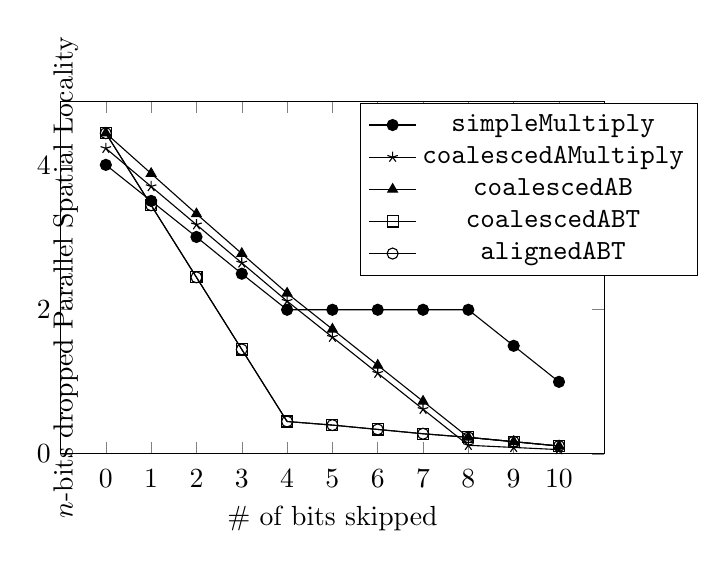
\begin{tikzpicture}
		\begin{axis}[symbolic x coords={0,1,2,3,4,5,6,7,8,9,10},
		width=0.7\textwidth,
		height=0.5\textwidth,
		xtick={0,1,2,3,4,5,6,7,8,9,10},
		xticklabel style={text height=2ex},
		ymin=0,
		ylabel={$n$-bits dropped Parallel Spatial Locality}, xlabel={\# of bits skipped},
		ylabel style={at={(axis description cs:0.05,.5)},anchor=south},
		legend entries={\texttt{simpleMultiply},\texttt{coalescedAMultiply},
			\texttt{coalescedAB}, \texttt{coalescedABT}, \texttt{alignedABT}},
		legend style={at={(0.55,0.75)},anchor=west}
		]
		
		\addplot[mark=*] coordinates {
			(0, 4.01)
			(1,3.51)
			(2,3.01)
			(3,2.50)
			(4,2.00)
			(5,2.00)
			(6,2.00)
			(7,2.00)
			(8,2.00)
			(9,1.5)
			(10,1.00)
		};
		
		
		\addplot[mark=star] coordinates {
			(0,4.24)
			(1,3.71)
			(2,3.18)
			(3,2.65)
			(4,2.12)
			(5,1.62)
			(6,1.12)
			(7,0.62)
			(8,0.12)
			(9,0.09)
			(10,0.06)
		};
		
		\addplot[mark=triangle*] coordinates {
			(0,4.45)
			(1,3.89)
			(2,3.33)
			(3,2.78)
			(4,2.23)
			(5,1.73)
			(6,1.23)
			(7,0.73)
			(8,0.23)
			(9,0.17)
			(10,0.11)
		};
		
		\addplot[mark=square] coordinates {
			(0,4.45)
			(1,3.45)
			(2,2.45)
			(3,1.45)
			(4,0.45)
			(5,0.40)
			(6,0.34)
			(7,0.28)
			(8,0.23)
			(9,0.17)
			(10,0.11)
		};
		
		\addplot[mark=o] coordinates {
			(0,4.45)
			(1,3.45)
			(2,2.45)
			(3,1.45)
			(4,0.45)
			(5,0.40)
			(6,0.34)
			(7,0.28)
			(8,0.23)
			(9,0.17)
			(10,0.11)
		};
		\end{axis}
		\end{tikzpicture}
		\caption{Calculated parallel spatial locality metric for matrix multiply kernels for 256 $\times$ 256 matrix multiplication}
		\label{fig: matmul parallel spatial locality}
	\end{figure*}
	
	There are three steps involved in generating an AIWC metric: \textit{recording}, \textit{calculating} and \textit{summarising} data collected from the symbolic execution of the kernel under inspection.
	
	\textit{Record}: we first record memory accesses performed by each thread in an OpenCL thread group as described above to achieve a global ordering of all memory accesses performed in a thread group. This ordering is collected in the form of logical timestamps ($t_0 .. t_{last}$) at which memory accesses occur.
	
	\textit{Calculate}: for each timestamp $t = t_0 .. t_{last}$, calculate the n-bits dropped entropy of memory addresses accessed by all threads in a work group within the timestamp $t$. Here $n$ can range between 1 and 10 as was the case for $LMAE$.
	
	\textit{Summarise}: average the collected entropy values across all the timestamps to calculate the parallel spatial locality metrics for one thread group. We then average the n-bits dropped entropy summaries across thread groups to obtain the \textit{n-bits dropped parallel spatial locality metrics} for the kernel's execution.
	
%	\begin{equation} \label{entropyaverage}
%		\log_2(\frac{\sum_{t = t_0}^{t_{last}} 2^{E_{n,t}}}{\#{timestamps}})
%	\end{equation} 
	
%	With $E_{n,t}$ the n-bits dropped entropy at timestamp $t$.

	The proposed metric is a parallel computing analogue for MICA's data stride metric that measures the distance between consecutive data accesses in a single threaded environment. In parallel programs, to accurately measure spatial locality of accesses, we must consider memory accesses performed by multiple threads in a close temporal scope. The proposed metric calculates the locality of accesses in each time step of the program's execution and steeper drop-offs in $n$-bits dropped parallel spatial locality scores will be observed in programs that access nearby memory addresses within the same timestamp. Such programs will perform better on GPUs, as they will make better use of both global memory access coalescing and shared memory bank structures.
	
	In figure \ref{fig: matmul parallel spatial locality} we see theoretical calculations for the proposed parallel spatial locality metric for each of the matrix multiplication kernels from section \ref{motivating example}. In particular we observe that the \texttt{coalescedABT} and \texttt{alignedABT} kernels have the steepest drop-offs in entropy as the number of bits skipped is increased, which correlates to better locality of parallel memory accesses. It is expected for these kernels to exhibit better parallel spatial locality than \texttt{simpleMultiply}, as \texttt{coalescedABT} and \texttt{alignedABT} make use of shared memory, where accesses tend to be localised simply due to the small size of shared on-chip memory typically available on GPUs. Further we find that the proposed metric successfully distinguishes between the \texttt{coalescedAB} and \texttt{coalescedABT} kernels. It accurately depicts a steeper drop-off for the more optimised \texttt{coalescedABT} kernel, where a larger proportion of parallel memory accesses make better use of the memory bank structure of GPU shared memory than all previous kernels. This is a significant improvement over the state-of-the-art AIWC metrics in characterising how codes localise shared memory accesses to better use the hardware provided.
	
	\section{Results}
	
	We present the results of running the AIWC tool on the Extended OpenDwarfs benchmark suite \cite{opendwarfs2017base,extendedopendwarfs}.
	
	\subsection{N-body methods: GEM}
	
	\subsection{Dense Linear Algebra: LUD}
	
	Lower-upper decomposition (LUD) in OpenDwarfs is a program to decompose an input square matrix as the product of one lower and one upper diagonal matrix. LUD is a Memory access patterns in a dense linear algebra workload such as LUD are typically highly regular and deterministic for each OpenCL work item, based on the the matrix dimension and offset parameters.
	
	The OpenDwarfs implementation \cite{opendwarfs2017base} splits the LUD computation into three kernels, ...  %TODO: Divergence in the kernels. Make a diagram/code simplification for LUD.
	
	\subsection{Structured Grids: SRAD}
	
	Speckle Reducing Anisotropic Diffusion (SRAD) attempts to remove locally correlated noise from images by following a repeated, structured grid update computation pattern. Conditional statements in the code cause thread divergence, potentially within a work-group, to handle boundary conditions. These boundaries constitute a small portion of the executed work-items, especially on larger data-sets and so the .
	
	\subsection{Graph Traversal: BFS}
	
	Graph traversal algorithms require pointer chasing operations to traverse nodes of a graph to perform calculations. The Breadth First Search 
	
	\section{Conclusions and Future Work} \label{future work}
	
	To the best of our knowledge this work is the first to critically examine architecture independent methods to measure memory access patterns and guide hardware-specific optimisation. We implemented and justified the addition of relative local memory usage to AIWC in our steps to characterise memory-based GPU code optimisations. We have also proposed the methodology to implement a new parallel spatial locality metric to AIWC. Upon implementation, our work would be the first to measure memory access patterns of parallel codes in an architecture-independent, easily interpreted manner.
	%TODO UPDATE IN FUTURE
	
	Our proposed parallel spatial locality metric may also correlate to some memory-based optimisation strategies for CPUs. Future work would apply the approach followed by this paper to CPU and FPGA architectures to evaluate the viability of an architecture independent characterisation of memory access patterns in codes targeted to these architectures.
	
	Future work will provide a concrete implementation of this new parallel spatial locality metric in the AIWC framework. It is then feasible to test these new metrics across a larger set of GPU targeted OpenCL codes. This will allow a critical examination of the effectiveness of both proposed metrics in accurately profiling memory access patterns of these diverse codes.

	\bibliographystyle{plain}
	\bibliography{bib/bibliography.bib}
	
	\begin{appendix}
		
		\section{\texttt{simpleMultiply} kernel} \label{simpleMultiply}
		
		\begin{lstlisting}
		__kernel void simpleMultiply(__global float *A,
				__global float *B, 
				__global float *C, 
				int N)
		{
			const int globalRow = get_global_id(0); // Row ID of C (0..N-1)
			const int globalCol = get_global_id(1); // Col ID of C (0..N-1)
			// Compute a single element of C (loop over K)
			float acc = 0.0f;
			for (int k = 0; k < N; ++k) {
				acc += B[k * N + globalCol] * A[globalRow * N + k];
		`	}
			// Store the result
			C[globalRow * N + globalCol] = acc;
		}
		
		\end{lstlisting}
		
		\section{\texttt{coalescedAMultiply} kernel} \label{coalescedAMultiply}

			
		\begin{lstlisting}
		__kernel void coalescedAMultiply(
				const __global float* A,
				const __global float* B,
				__global float* C,
				const int N)
		{
			__local float aTile[TILE_DIM][TILE_DIM];
			
			const int localRow = get_local_id(0);
			const int localCol = get_local_id(1);
			
			const int globalRow = get_global_id(0);
			const int globalCol = get_global_id(1);
			
			__private float sum = 0.0f;
			
			const int numTiles = N / TILE_DIM;
			__private const int tiledRow = globalRow*N+ localCol;
			for (int i = 0; i < numTiles; i++) {
				aTile[localRow][localCol] = A[tiledRow+i*TILE_DIM];
				barrier(CLK_LOCAL_MEM_FENCE);
				for (int k = 0; k < TILE_DIM; k++) {
					sum += aTile[localRow][k] * B[(i*TILE_DIM+k)*N+globalCol];
				}
				barrier(CLK_LOCAL_MEM_FENCE);
			}
			C[globalRow*N+globalCol] = sum;
		}
		\end{lstlisting}

		
		\section{\texttt{coalescedAB} kernel} \label{coalescedABMultiply}
			
		\begin{lstlisting}
		__kernel void coalescedAB(
				const __global float* A,
				const __global float* B,
				__global float* C,
				const int N) {
			__local float ASub[TILE_DIM][TILE_DIM];
			__local float BSub[TILE_DIM][TILE_DIM];    
			
			const int localRow = get_local_id(0);
			const int localCol = get_local_id(1);
			const int globalRow = get_global_id(0);
			const int globalCol = get_global_id(1);
			
			float acc = 0.0f;
			const int numTiles = N/TILE_DIM;
			
			for (int i = 0; i < numTiles; i++) {
				const int tiledRow = globalRow*N+i*TILE_DIM + localCol;
				const int tiledCol = globalCol + (TILE_DIM*i + localRow)*N;
				ASub[localRow][localCol] = A[tiledRow];
				BSub[localRow][localCol] = B[tiledCol];
				
				barrier(CLK_LOCAL_MEM_FENCE);
				
				for (int k=0; k<TILE_DIM; k++) {
					acc += ASub[localRow][k] * BSub[k][localCol];
				}
				
				barrier(CLK_LOCAL_MEM_FENCE);
			}
			C[globalRow*N + globalCol] = acc;
		}
		\end{lstlisting}
	\end{appendix}
	
\end{document}